
\chapter{Surface and Triple Integrals}

This chapter covers the following ideas. 

% A list of objectives for the chapter
%\begin{enumerate}
%\item ...
%\end{enumerate}


\begin{enumerate}
\item Explain how to setup surface integrals, as well as how to
compute surface area.
\item Explain how to set up and compute triple
  integrals, as well as how to interchange the bounds of
  integration. Use these ideas to find volume.
\item For surfaces and solid regions, find area,
  mass, centroids, center of mass, moments of interia, and radii of
  gyration.
\item Explain how to change coordinate systems in integration, in
  particular to polar, cylindrical, and spherical coordinates. Explain
  what the Jacobian of a transformation is and how to use it.
\end{enumerate}

%%% Local Variables: 
%%% mode: latex
%%% TeX-master: "../multivariable-calculus"
%%% End: 
%$

\section{Surface Area and Surface Integrals}
\prepproblems{14.5: 11, 17, 31\\
15.5: 37}%
Recall that the line integral $\int_C 1 ds$ gives arc length of a curve
$C$ and is an extension of the single integral $\int_a^b 1 dx$ which
gives the length of $[a,b]$.  Similarly, we will define the integral
$\iint_S 1 d\sigma$ to give surface area of a surface $S$, which is an
extension of the double integral $\iint_R 1 dA$ which gives area of a
region $R$.

We start by finding the surface area of the surface {$S: z=f(x,y) $}
for $(x,y)$ in some region $R$. The idea is to add up little pieces of
surface area. Divide $R$ into a tiny grid in which each little
rectangle has dimensions $\Delta x$ and $\Delta y$. Since $f$ is differentiable,
it can be approximated on a small region by the tangent plane.  In
this tangent plane, the portion of the surface above a tiny rectangle
is a parallelogram.  The vectors $\langle1,0,f_x\rangle\Delta x$ and
$\langle0,1,f_y\rangle\Delta x$ represent the edges of the
parallelogram. The area of the parallelogram is the magnitude of their
cross product, which is $|\langle-f_x,-f_y,1\rangle\Delta x\Delta y| =
\sqrt{f_x^2+f_y^2+1}$. A little piece of surface area is approximated
using the formula $d\sigma = \sqrt{f_x^2+f_y^2+1}dA$. Surface area is found
by adding up little bits of surface area, hence {$ \sigma=\iint_S d\sigma =
  \iint_R \sqrt{f_x^2+f_y^2+1} dA $} where {$S$} stands for the
surface, and {$R$} stands for the shadow of the surface in the
{$xy$}-plane.

If the surface is given by the parametrization $S:\vec
r(u,v)=\langle x,y,z\rangle$ for $(u,v)$ in some region $R$ in the $uv$
plane, then let $\Delta u$ and $\Delta v$ be small changes in the inputs $u$ and
$v$ (this places a grid on $R$). A portion of the surface
corresponding to a tiny change in $u$ and $v$ is approximately a
parallelogram, whose edges are given by the vectors $\vec r_u \Delta u$ and
$\vec r_v\Delta v$. The magnitude of the cross product of these two vectors
is, in differential notation, $d\sigma = |\vec r_u\times \vec r_v|dudv $. Total
surface area is found by adding up little bits of surface area, giving
the integral formula $\sigma=\iint_S d\sigma = \iint_R |\vec r_u\times \vec
r_v|dudv$. Notice that if the surface is $z=f(x,y)$, then a
parametrization is $\vec r(x,y)=\langle x,y,f(x,y)\rangle$, so $|\vec
r_x\times \vec r_y|dxdy = |\langle1,0,f_x\rangle\times \langle0,1,f_y\rangle|dxdy
= \sqrt{f_x^2+f_y^2+1} dA$.  For a surface $y=f(x,z)$, the
parametrization $\vec r(x,z)=\langle x,f(x,z),z\rangle$ gives $d\sigma =
\sqrt{f_x^2+1+f_z^2} dxdz$. Likewise $d\sigma = \sqrt{1+f_y^2+f_z^2} dydz$
for a surface $x=f(y,z)$.

\begin{example}
  Consider the surface $S:z=9-x^2-y^2$ for $x^2+y^2\leq 9$. We compute
  $\sqrt{f_x^2+f_y^2+1} = \sqrt{4x^2+4y^2+1}$. Surface area is
  $\sigma=\iint_S d\sigma = \int_{-3}^{3}\int_{-\sqrt{9-x^2}}^{\sqrt{9-x^2}}
  \sqrt{4x^2+4y^2+1} dydx$. Converting to polar coordinates gives
  $\int_{0}^{2\pi}\int_{0}^{3} \sqrt{4r^2+1}r drd\theta$, which is an integral we
  can compute (letting $u=4r^2+1$). The same surface can be
  parametrized as $\vec r(r,\theta) = \langle r\cos \theta,r\sin \theta, 9-r^2\rangle$
  for $0\leq r\leq 3$ and $0\leq \theta \leq 2\pi$. We calculate $|\vec r_r\times \vec r_\theta| =
  |\langle\cos \theta,\sin \theta, -2r\rangle\times \langle-r\sin \theta,r\cos \theta, 0\rangle|
  = |\langle2r^2\cos \theta, 2r^2\sin \theta, r\cos^2
    \theta+r\sin^2\theta\rangle|=|\langle2r^2\cos \theta, 2r^2\sin \theta,r\rangle| =
  \sqrt{4r^4+r^2} = r\sqrt{4r^2+1}$.  Hence we have $d\sigma =
  r\sqrt{4r^2+1}drd\theta$ as before, which means $\sigma = \int_{0}^{2\pi}\int_{0}^{3}
  \sqrt{4r^2+1}r drd\theta$. Notice that you get the same answer in two
  different ways.
\end{example}


\begin{example}
If a surface consists of many different pieces (a cube has 6 faces),
then a surface integral over such a surface is the sum of the
integrals over each of the surfaces. To integrate the function
$g(x,y,z)=yz$ over the surface of the wedge in the first octant
bounded by the coordinate planes and the planes $x=2$ and $y+z=1$, we
notice that the surface has 5 parts.  The portions are $S_1$: $x=0$ for
$0\leq y\leq 1$, $0\leq z\leq 1-y$;  $S_2$: $x=2$ for $0\leq y\leq 1$, $\leq z\leq 1-y$;
$S_3$: $y=0$ for $0\leq x\leq 2$, $0\leq z\leq 1$; $S_4$: $z=0$ for $0\leq x\leq 2$, $0\leq y\leq 1$; and
$S_5$: $z=1-y$ for $0\leq x\leq 2$, $0\leq y\leq 1$. Hence, to find $\iint_S g d\sigma$, we
must evaluate all 5 integrals.  We compute $d\sigma_1 = \sqrt{1+0+0}dzdy$,
$d\sigma_2=\sqrt{1+0+0}dzdy$, $d\sigma_3=\sqrt{0+1+0}dzdx$, $d\sigma_4=\sqrt{0+0+1}dydx$, $d\sigma_5=\sqrt{0+(-1)^2+1}dydx$, and so 
$$\begin{array}{llllll}
&\iint_{S_1} g d\sigma&+\iint_{S_2} g d\sigma&+\iint_{S_3} g d\sigma&+\iint_{S_4} g
d\sigma&+\iint_{S_5} g d\sigma\\
=&\int_0^1\int_{0}^{1-y} yz dzdy&+\int_0^1\int_{0}^{1-y} yz dzdy&+\int_0^2\int_{0}^{1}
(0)z dzdx&+\int_0^2\int_{0}^{1} y(0) dydx&+\int_0^2\int_{0}^{1} y(1-y)
\sqrt{2}dydx\\
=&\int_0^1\int_{0}^{1-y} yz dzdy&+\int_0^1\int_{0}^{1-y} yz
dzdy&+0&+0&+\int_0^2\int_{0}^{1} y(1-y) \sqrt{2}dydx\\
=&1/24&+1/24&+0&+0&+\sqrt{2}/3
\end{array}$$
\end{example}




\subsection{Physical Applications}
\prepproblems{15.6: 5, 11, 15}%
Integrals are used in a wide variety of applications.  You should
notice that in most of the applications below, a formula which works
for a surface integral is the same as the double integral and line
integral formulas.  The differentials $dx,ds,dA,d\sigma$ remind us which
type of integral to use.  For lack of a better notation,  I will use
$d\square$ to represent any of these differentials when you are free
to pick the needed differential. I start by giving a summary of the
differential formulas, and then we will use them to find some physical
quantities.
\begin{itemize}
\item Area: $dA = fdx,fds, dxdy, rdrd\theta, \frac{\partial(x,y)}{\partial(u,v)}dudv$, 
\item Surface Area: $|\vec r_u\times\vec r_v|dudv = d\sigma =
\sqrt{f_x^2+f_y^2+1}dxdy = \sqrt{f_x^2+1+f_z^2}dxdz =
\sqrt{1+f_y^2+f_z^2}dydz $
\item Volume: $dV = fdA = fd\sigma$, 
%\item Flux: $d\text{Flux} = \vec F\cdot \vec n d\sigma ,  \vec F\cdot \vec n ds$
%where $\vec n$ is a unit normal vector to either a surface $S$ or a curve
%$C$.
\item Average Value: $(\bar f)\square = \int fd\square$, 
\item Mass: $dm = \delta d\square , \delta dx, \delta ds, \delta dA, \delta d\sigma$
\item Center of Mass: $(\bar x,\bar y,\bar z)m = \int\langle x,y,z\rangle
dm$, where $\int \bar x dm = \int x dm$ is a first moment of mass
\item Moment of Inertia: $I = \int r^2 dm$ is a moment of inertia, and $\int
R^2 dm = \int r^2 dm$ gives $R^2 m =I$ or $R=\sqrt{I/m}$
\end{itemize}
I strongly suggest that as you do each problem, start from a formula
in differential notation, and then modify it so that you have the
right number of integrals.  If you do this, you will learn how to do
calculus in all dimensions with ease.


\begin{example}
  The temperature at each point in space on the surface of a sphere of
  radius 3 is given by {$T(x,y,z) = \sin(xy+z)$}. The average
  temperature on the sphere is given by the surface integral $AV =
  \frac{1}{\sigma}\iint_S fd\sigma$. A parametrization of the surface
  is {$\vec r (\theta,\phi) =
    \langle3cos\theta\sin\phi,3\sin\theta\sin\phi,3\cos\phi\rangle$}
  for {$0\leq \theta\leq 2\pi$} and {$0\leq \phi\leq \pi$}. We have
  {$T(\theta,\phi) =
    \sin((3\cos\theta\sin\phi)(3\sin\theta\sin\phi)+3\cos\phi)$}, and
  the surface area differential is {$d\sigma = |\vec
    r_\theta\times\vec r_\phi| = 9\sin \phi$}. The surface area is
  $\sigma = \int_{0}^{2\pi} \int_{0}^{\pi} 9\sin \phi d\phi d\theta$
  and the average temperature on the surface is $AV =\frac{1}{\sigma}
  \int_{0}^{2\pi} \int_{0}^{\pi}
  \sin((3\cos\theta\sin\phi)(3\sin\theta\sin\phi)+3\cos\phi) 9\sin
  \phi d\phi d\theta $.
\end{example}

\begin{example}
  Consider the surface which is the upper hemisphere of radius 3.  A
  parametrization of the surface is {$\vec r (\theta,\phi) =
    \langle3\cos\theta\sin\phi,3\sin\theta\sin\phi,3\cos\phi\rangle$}
  for {$0\leq \theta\leq 2\pi$} and {$0\leq \phi\leq \pi/2$}. The
  surface area differential is {$d\sigma = |\vec r_\theta\times\vec
    r_\phi|d\theta d\phi = 9\sin \phi d\theta d\phi$}. The surface
  area is $\sigma = \int_{0}^{2\pi} \int_{0}^{\pi/2} 9\sin \phi d\phi
  d\theta$. If the density is $\delta(x,y,z) = z^2$, then we have
  \begin{align*}
    \bar y &= \frac{\int y dm}{\int dm}= \frac{\iint_S y \delta
      d\sigma}{\iint_S \delta d\sigma} = \frac {\int_{0}^{2\pi}
      \int_{0}^{\pi/2} (3\sin\theta\sin\phi)(3\cos\phi)^2(9\sin \phi)
      d\phi d\theta}
    {\int_{0}^{2\pi} \int_{0}^{\pi/2} (3\cos\phi)^2(9\sin \phi) d\phi d\theta}\\
    R_y &= \sqrt{\frac{\int r^2 dm}{\int dm}} =\sqrt{\frac{\int
        x^2+z^2 dm}{\int dm}} = \sqrt{\frac {\int_{0}^{2\pi}
        \int_{0}^{\pi/2}[(3\cos\theta\sin\phi)^2+(3\cos\phi)^2]
        (3\cos\phi)^2(9\sin \phi) d\phi d\theta} {\int_{0}^{2\pi}
        \int_{0}^{\pi/2} (3\cos\phi)^2(9\sin \phi) d\phi d\theta}}
  \end{align*}
\end{example}




\section{Triple Integrals}
\prepproblems{14.6: 17, 23, 29}%
The triple integral of a function $f(x,y,z)$ over a solid region $D$
in space, written $\iiint_D f dV$, is defined similarly as a double
integral.  We break a region in space up into little boxes of
dimensions $\Delta x,\Delta y, \Delta z$, and then take a limit of the sum $\sum\sum\sum f\Delta x\Delta
y \Delta z$ to get the triple integral. If the function is $f=1$, then this
integral gives the volume of the region $D$ in space. Since there are
six ways to order $x$, $y$, and $z$, there are six different iterated
integrals which can be used to compute a triple integral. Sometimes
one order to use is easier than another.  Which one to use will come
with practice. Make sure you tackle the problems in the text which ask
you to write an integral in six different ways. You have to pick an
outside, middle, and inner variable in any case.  The outside variable
is bounded between two constants, representing two parallel planes
which bound the region $D$.  The middle variable is bounded between
two functions of the outer variable.  These two middle functions
represent two cylinders which bound the solid region $D$ (not circular
cylinders, but generic cylinders which are parallel to the inner
variable axis). The inner variable is bounded between two functions of
the outer and middle variables, and represent two surfaces which bound
region $D$. 

\begin{wrapfigure}[6]{l}[24pt]{0pt}
\newcommand{\myheight}{.8in}
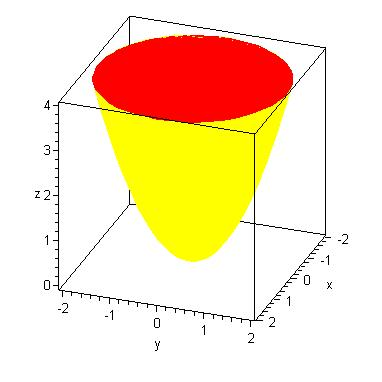
\includegraphics[height=\myheight]{10-SurfaceTripleIntegrals/support/triple-1}
\end{wrapfigure}
The region above the paraboloid $z=x^2+y^2$ below the plane $z=4$ has
$x$ values between $-2$ and $2$ (the outer bounds). The $y$ values lie
in the cylinder $x^2+y^2=4$ or $y=-\sqrt{4-x^2}$ and $y=\sqrt{4-x^2}$.
The $z$ values lie between the surfaces $z=x^2+y^2$ and $z=4$.  So we
have for our bounds the inequalities $-2\leq x\leq 2$, $-\sqrt{4-x^2}\leq y\leq
\sqrt{4-x^2}$, and $x^2+y^2\leq z\leq 4$ (planes, cylinders, surfaces) which
can be used to find the volume of this region by the triple integral
$V=\int_{-2}^{2}\int_{-\sqrt{4-x^2}}^{\sqrt{4-x^2}}\int_{x^2+y^2}^{4}1 dz dy
dx$. This integral is rather complicated to solve by hand as written,
but using an appropriate high dimensional change of coordinates, this
integral becomes rather trivial.  Spend most of your time learning to
set up integrals rather than solving them.

\begin{wrapfigure}[6]{l}[24pt]{0pt}
\newcommand{\myheight}{.8in}
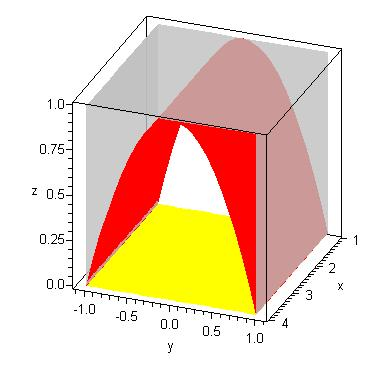
\includegraphics[height=\myheight]{10-SurfaceTripleIntegrals/support/triple-2}
\end{wrapfigure}
The region $D$ below the cylinder $z=1-y^2$ above the $xy$ plane and
between the planes $x=1,x=4$ can be found as follows.  If we choose
$x,y,z$, as our outer, middle, inner bounds, then $1\leq x\leq 4,-1\leq y\leq 1,0\leq
z\leq 1-y^2$.  If we choose instead the order $z,x,y$, then we have $0\leq
z\leq 1$, $1\leq x\leq 4$, and $-\sqrt{1-z}\leq y\leq \sqrt{1-z}$ (just solve for $y$
in the equation $z=1-y^2$ to find the bounds for $y$).  Hence the
volume of this region can be written two ways as
$V=\int_{1}^{4}\int_{-1}^{1}\int_{0}^{1-y^2}1 dz dy dx =
\int_{0}^{1}\int_{-1}^{1}\int_{-\sqrt{1-z}}^{\sqrt{1-z}}1 dy dx dz$. 

We currently have two ways of finding volume, either $\iint_R fdA$ or
$\iiint_D 1 dV$.  Using differential notation $dA=fdx=dxdy$ and $dV =
fdA = fdxdy = dxdydz$ helps remind us of how to find area and volume
in any manner.  The formula $dA=fdx$ reminds us that little pieces of
area can be found by taking a height times a little change in $x$ and
using a single integral.  The formula $dA = dxdy$ reminds us that area
can also be found using a double integral as area is little changes in
width times little changes in length.  Similarly $dV=fdA=fdxdy$
reminds us that volume can be found using a double integral, or
$dV=dxdydz$ says that volume can be found using a triple integral.
The shell method $dV=2\pi xf(x)dx$ and disk method $dV = \pi (f(x))^2dx$
can also be summarized in differential notation, and since there is
only $dx$ you only use a single integral.  If you can remember how to
compute a little piece of volume $dV$ using any of these formulas,
then total volume is found by adding up all the little pieces. The
number of integrals used depends on the number of differentials like
$dx$, $dy$, or $dz$. If you use a single integral sign to represent
however many iterated integrals you need (depending on the
differential), then you can write area as ``add up little bits of
area'' ($A=\int_RdA$), and volume as ``add up little bits of volume''
($V=\int_D dV$), where the number of integrals is determined by the
differential formula you choose for $dA$ or $dV$.

\section{Changing Coordinate Systems---Generalized $u$-substitution}
\prepproblems{14.7: 13, 19\\14.8: 27}%
Just as we did with polar coordinates in two dimensions, we can
compute a Jacobian for any change of coordinates in three dimensions.
We will focus on cylindrical and spherical coordinate systems.
Remember that the Jacobian of a transformation is the absolute value
of the determinant of the derivative of the transformation.

\subsection{Cylindrical Coordinates}
Cylindrical coordinates are defined by $x=r\cos\theta$, $y=r\sin\theta$, and
$z=z$, which we can represent using function notation as
$T(r,\theta,z)=\langle r\cos\theta, r\sin\theta,z\rangle$. The derivative of this transformation
is 
$DT(r,\theta,z)= 
\begin{bmatrix}
\cos\theta&-r\sin\theta&0\\
\sin\theta&r\cos\theta&0\\
0&0&1
\end{bmatrix}$. The Jacobian of the transformation is
$\frac{\partial(x,y,z)}{\partial(r,\theta,z)} = |\det(DT(r,\theta,z))| = |r|$. Provided that
$r\geq 0$, we have the differential formula $dV=rdrd\theta dz$, or in integral
form the equation $\iiint_{D_{xyz}} f(x,y,z)dxdydz = \iiint_{D_{r\theta z}}
f(T(r,\theta,z))\frac{\partial(x,y,z)}{\partial(r,\theta,z)}drd\theta dz=  \iiint_{D_{r\theta z}}
f(T(r,\theta,z))(r)drd\theta dz $. In summary, converting to cylindrical
coordinates requires that we multiply by $r$. Cylindrical coordinates
are extremely useful for problems which involve cylinders,
paraboloids, and cones. 

\begin{wrapfigure}[6]{l}[24pt]{0pt}
\newcommand{\myheight}{.8in}
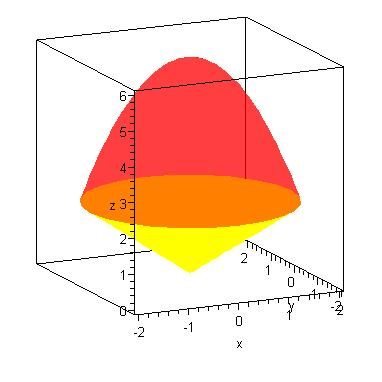
\includegraphics[height=\myheight]{10-SurfaceTripleIntegrals/support/cylindrical-1}
\end{wrapfigure}
We now find the volume of the region $D$ in space which is above the
cone $z=\sqrt{x^2+y^2}$ and below the paraboloid $z=6-x^2-y^2$.
Switching to cylindrical coordinates, these equations become $z=r$ for
the cone and $z=6-r^2$ for the paraboloid.  The surfaces intersect
when $r=6-r^2$, or $r^2+r-6 = (r+3)(r-2)=0$, or $r=2,-3$. Since $z>0$,
we know that the intersection we seek is at $r=2$. So the region $D$
in space is the set of points above $z=r$, below $z=6-r^2$, and inside
the cylinder $r=2$.  We can describe this region using the
inequalities $0\leq \theta\leq 2\pi$, $0\leq r\leq 2$, and $r\leq z\leq 6-r^2$. This gives us
the volume as $V = \int_0^{2\pi}\int_0^2\int_r^{6-r^2}(r)dzdrd\theta$. 

\begin{wrapfigure}[6]{l}[24pt]{0pt}
\newcommand{\myheight}{.8in}
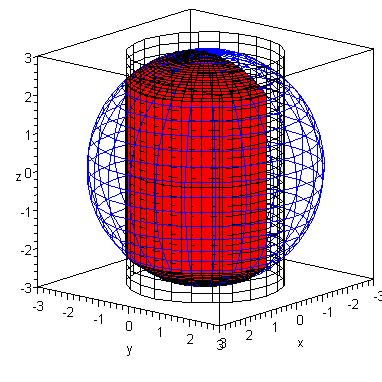
\includegraphics[height=\myheight]{10-SurfaceTripleIntegrals/support/cylindrical-2}
\end{wrapfigure}
The integral
$\int_0^2\int_{-\sqrt{4-x^2}}^{\sqrt{4-x^2}}\int_{-\sqrt{9-x^2-y^2}}^{\sqrt{9-x^2-y^2}}dzdydx$
represents the volume of the region in space satisfying the
inequalities $0\leq x\leq 2$, ${-\sqrt{4-x^2}}\leq y\leq {\sqrt{4-x^2}}$, and
${-\sqrt{9-x^2-y^2}}\leq z\leq{\sqrt{9-x^2-y^2}}$, or the region in space
with positive $x$ values inside the cylinder $x^2+y^2=4$ and inside
the sphere $x^2+y^2+z^2=9$. Since this problem involves a cylinder, we
will write the integral in cylindrical coordinates.  The region is
described using $-\pi/2\leq \theta\leq \pi/2$, $0\leq r\leq 2$, and $-\sqrt{9-r^2}\leq z\leq 
\sqrt{9-r^2}$, which means that we can rewrite the integral as $V=
\int_{-\pi/2}^{\pi/2}\int_0^2\int_{-\sqrt{9-r^2}}^{\sqrt{9-r^2}}(r)dzdrd\theta $. The
volume of the region outside the cylinder of radius 2, inside the
sphere of radius 3, with positive $x$ values is given by either $V=
\int_{-\pi/2}^{\pi/2}\int_2^3\int_{-\sqrt{9-r^2}}^{\sqrt{9-r^2}}(r)dzdrd\theta $ or $V=
\int_{-\pi/2}^{\pi/2}\int_{-\sqrt 5}^{\sqrt{5}}\int_{2}^{\sqrt{9-z^2}}(r)drdzd\theta $
(since the cylinder intersects the sphere at a height of $\sqrt 5$).



\subsection{Spherical Coordinates}
Spherical coordinates are defined by $T(\rho,\theta,\phi) = \langle\rho\cos\theta\sin\phi,
\rho\sin\theta\sin\phi,\rho\cos\phi\rangle$.  The Jacobian of this transformation is $\ds
\frac{\partial(x,y,z)}{\partial(\rho,\theta,\phi)} = |\det(DT(\rho,\theta,\phi)| = |-\rho^2\sin\phi|$ (verify
this as homework). Using differential notation, we write
$dV=dxdydz=|\rho^2\sin\phi|d\rho d\theta d\phi$, so that whenever you convert to
spherical coordinates from rectangular, you have to multiply by
$|\rho^2\sin\phi|$ inside the integral, or just $\rho^2\sin\phi$ if you require
{$0\leq \phi\leq \pi$}. Problems which involve cones and spheres often have
simple integrals in spherical coordinates.

The volume inside a sphere of radius $a$ is
$\int_{-a}^{a}\int_{-\sqrt{a^2-x^2}}^{\sqrt{a^2-x^2}}\int_{-\sqrt{a^2-x^2-y^2}}^{\sqrt{a^2-x^2-y^2}}dzdydx$.
This integral is rather difficult to solve by hand (if it is even
possible).  However the region inside the sphere is describe in
spherical coordinates as $0\leq \phi \leq \pi$, $0\leq \theta\leq 2\pi$, and $0\leq \rho\leq a$.  Hence
the volume is found using $V=\int_0^\pi\int_0^{2\pi}\int_0^a \rho^2\sin\phi d\rho d\theta d\phi$.
This integral can be evaluated using elementary techniques and gives
the volume $V=\frac{4}{3}\pi a^3$.


\begin{wrapfigure}[5]{l}[24pt]{0pt}
\newcommand{\myheight}{.8in}
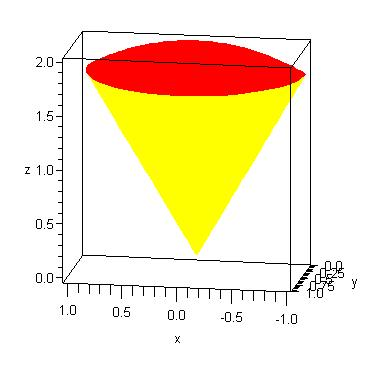
\includegraphics[height=\myheight]{10-SurfaceTripleIntegrals/support/spherical-1}
\end{wrapfigure}
The integral $\int_{0}^{\pi}\int_{0}^{1}\int_{\sqrt{3}r}^{\sqrt{4-r^2}}rdzdrd\theta$
represents the region in space with $y\geq 0$, $r\leq 1$, above the cone
$z=\sqrt 3 r$, and below the sphere $z^2=4-r^2$. The cone and sphere
intersect precisely when $r=1$.  In rectangular coordinates, the
integral is
$\int_{-1}^{1}\int_{0}^{\sqrt{1-x^2}}\int_{\sqrt{3(x^2+y^2)}}^{\sqrt{4-x^2-y^2}}dzdydx$. 
In spherical coordinates, the cone is given by the equation $\phi=\pi/6$
(draw a right triangle with hypotenuse 2 and one side length 1), and
the sphere is given by the equation $\rho = 2$. The integral becomes
$\int_{0}^{\pi}\int_{0}^{\pi/6}\int_{0}^{2}\rho^2\sin\phi d\rho d\phi d\theta$. 









\section{Physical Applications}
\prepproblems{14.6: 33, 49, 63\\ 14.7: 21, 35}%
Integrals are used in a wide variety of applications.  Notice that in
all of the applications we have done this semester, a formula which
works for double integrals will also work for single, line, surface,
and triple integrals.  The differentials $dx,ds,dA,d\sigma, dV$ remind us
which dimension we are working in.  For lack of a better notation,  I
will use $d\square$ to represent any of these differentials when you
are free to pick the needed differential. The line integrals section
contains the details for each of the physical quantities we compute.


\subsection{The Short Version}
Everything we learned about physical applications this semester can be
summarized in the following table list, where recall that $d\square$
stands for any of $dx,ds,dA,d\sigma,dV$.
\begin{itemize}
\item Area: $dA = fdx,fds, dxdy, rdrd\theta, \frac{\partial(x,y)}{\partial(u,v)}dudv$, 
\item Volume: $dV = fdA,dxdydz, rdrd\theta dz, \rho^2\sin\phi d\rho d\theta d\phi,
\frac{\partial(x,y,z)}{\partial(u,v,w)}dudvdw$, 
\item Surface Area: $d\sigma = |\vec r_u\times \vec r_v|dudv =
\sqrt{f_x^2+f_y^2+1}dxdy$
\item Average Value: $\bar f\square = \int fd\square$, and $dm = \delta
d\square , \delta dx, \delta ds, \delta dA, \delta d\sigma, \delta dV $
\item Center of Mass: $(\bar x,\bar y,\bar z)m = \int(x,y,z) dm$, where
$\int \bar x dm = \int x dm$ is a first moment of mass
\item Moment of Inertia: $I = \int rad^2 dm$ is a moment of inertia, and
$\int R^2 dm = \int r^2 dm$ gives $R^2 m =I$ or $R=\sqrt{I/m}$. Recall that
$rad^2 = y^2+z^2$ for $I_x$, $rad^2=x^2+z^2$ for $I_y$, and
$rad^2=x^2+y^2$ for $I_z$.
%\item Flux: $d\text{Flux} = \vec F\cdot \vec n d\sigma $ or $ \vec F\cdot \vec n
%ds$ where $\vec n$ is a normal vector to either a surface $S$ or a
%curve $C$.
%\item Circulation: $d\text{Circ} = \vec F\cdot \vec T ds  = Mdx+Ndy$.
\end{itemize}
I strongly suggest that as you do each problem, start from a formula
in differential notation, and then modify it so that you have the
right number of integrals.  If you do this, you will learn how to do
calculus in all dimensions with ease. 

\begin{example}
  Consider the region in space inside the cylinder $r=4$ bounded above
  by the cone $z=r$ and below by the $xy$-plane.  Using cylindrical
  coordinates, we have $dV = rdzdrd\theta$. The volume is
  $\int_{0}^{2\pi}\int_0^4\int_0^r rdzdrd\theta$.  If the density is
  $\delta(x,y,z) =x^2+z$, then we have
  \begin{align*}
    \bar y &= \frac{\int y dm}{\int dm}= \frac{\iiint_D y \delta
      dV}{\iiint_D \delta dV}= \frac{\int_{0}^{2\pi}\int_0^4\int_0^r
      r\sin\theta((r\cos\theta)^2+z)rdzdrd\theta}
    {\int_{0}^{2\pi}\int_0^4\int_0^r ((r\cos\theta)^2+z) rdzdrd\theta}\\
    R_z &= \sqrt{\frac{\int r^2 dm}{\int dm}} =\sqrt{\frac{\int
        x^2+y^2 dm}{\int dm}} = \sqrt{\frac
      {\int_{0}^{2\pi}\int_0^4\int_0^r((r\cos\theta)^2+(r\sin\theta)^2)
        ((r\cos\theta)^2+z) rdzdrd\theta}
      {\int_{0}^{2\pi}\int_0^4\int_0^r ((r\cos\theta)^2+z)
        rdzdrd\theta}}
  \end{align*}
\end{example}

\begin{example}
  The temperature at each point in space of a solid covering the
  region {$D$} (the upper portion of the sphere of radius 4 centered
  at the origin) is given by $T(x,y,z) = \sin(xy+z)$.  The volume and
  average temperature are

\begin{align*}
  V&=\int_{-4}^{4} \int_{-\sqrt{16-x^2}}^{\sqrt{16-x^2}}
  \int_{0}^{\sqrt{16-x^2-y^2}} dz dy dx\\
  AV&=\frac{1}{V}\int_{-4}^{4} \int_{-\sqrt{16-x^2}}^{\sqrt{16-x^2}}
  \int_{0}^{\sqrt{16-x^2-y^2}} \sin(xy+z) dz dy dx.
\end{align*}
\end{example}





%%% Local Variables: 
%%% mode: latex
%%% TeX-master: "../multivariable-calculus"
%%% End: 





